\documentclass[12pt]{article}
\usepackage{minted}
\usepackage{graphicx}
\usepackage{mathtools}
\usepackage{amsfonts}

\begin{document}
    \title{CS 541 Homework 4}
    \author{Stephen Szemis}
    \date{ December 5, 2020}
    \maketitle

    \paragraph{Part 1: Data Set}~\\
    temp

    \paragraph{Part 2: Learning}
    \subparagraph{1. Derive the gradients}
    We start with out original equation
    \[
        \operatorname*{min}_{U,V} F(U, V) :=
        \frac{1}{2} \sum_{(i,j) \in \Omega_{1}} (M_{ij} - u_i v_j^T)^2 
        + \frac{\lambda}{2} \bigl( \parallel U \parallel_{F}^{2} + \parallel V \parallel_{F}^{2} \big)
    \]
    We will look at each part of our derivative individually, as it can be complex to try to derive the answer in one 
    big step. Importantly the derivative of sums is the sum of derivatives. So we can look at each element of our Summation, and 
    try to see what the final partial might be.
    \[
        z_{ij} = \sum_{(i,j) \in \Omega_{1}} (M_{ij} - u_i v_j^T)^2 \, \text{for some i and j}
    \]
    We use the chain rule to get the "partial" solution\dots
    \[
        \frac{\partial z_{ij}}{\partial U} = -2(M_{ij} - u_{i}v_{j}^{T})V
    \]
    \[
        \frac{\partial z_{ij}}{\partial V} = -2(M_{ij} - u_{i}v_{j}^{T})U
    \]
    The other part of our original equation is easier to solve for.
    \[
        y = \frac{\lambda}{2} \bigl( \parallel U \parallel_{F}^{2} + \parallel V \parallel_{F}^{2} \big)
    \]
    Using the rules for the derivative of a Frobenius norm and chain rule we find\dots
    \[
        \frac{\partial y}{\partial V} = \lambda U
    \]
    \[
        \frac{\partial y}{\partial U} = \lambda V
    \]
    Finally putting it all together we get.
    \[
        \frac{\partial F(U, V)}{\partial U} = V\sum_{(i,j) \in \Omega_{1}} (M_{ij} - u_i v_j^T) + \lambda U
    \]
    \[
        \frac{\partial F(U, V)}{\partial U} = U\sum_{(i,j) \in \Omega_{1}} (M_{ij} - u_i v_j^T) + \lambda V
    \]

    \subparagraph{2. Lambda is 1}
    You can explore the code on the final pages of this report to see how this is implemented.
    Our update step is obviously just using the gradients above and updating each "row" of our U and V matrixes.
    The learning rate was a serious challenge for this entire assignment for me. I had a lot of trouble with
    overflow errors and had to more or less choose learning rates to stop this. Clearly I was finding some 
    bad behavior from my code. The learning rates in my final version run and give "fine" results, but I have a feeling
    I'm missing something about the relation between lambda and the learning rate. My graphs for part 2 are below.
    \begin{center}
    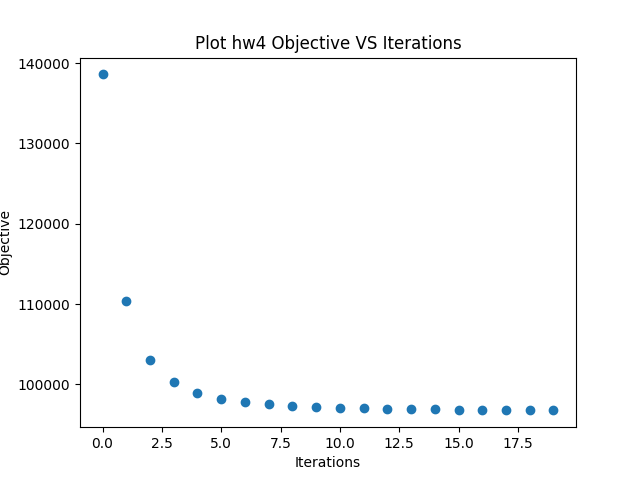
\includegraphics[width=12cm]{hw4_part2.png}
    \end{center}
    As you can see, we get a very nice move towards a minimum.

    \paragraph{Part 3: Evalutation}~\\
    The graph is below, as discuss in the last problem, I had issue with overflow errors and therefore I don't think
    my data is a very good reflection of how lambda changes behavior. Even so, this is what I ended up with.
    \begin{center}
    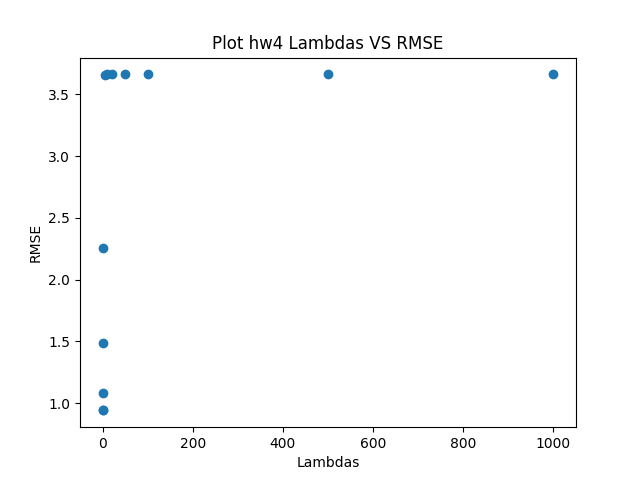
\includegraphics[width=12cm]{hw4_part3.png}
    \end{center}
    As you can see, lambda's that are lower have a much better error rate, but this might be due to the number of iterations 
    being low, or my learning rate being wrong.

    My code is below:
    \inputminted{python}{Szemis_hw4.py}

\end{document}